\documentclass{article}
\usepackage{amsmath}
\usepackage{geometry}
\usepackage{float}
\geometry{a4paper, left=2cm, right=2cm, top=2.54cm, bottom=2.54cm}
\usepackage{indentfirst}
\usepackage{enumitem}
\usepackage{bm}
\usepackage[hidelinks]{hyperref}

% 段落間距  (begin doc 才設定)
\usepackage{parskip}
    % 普通文字,行距
    \usepackage[onehalfspacing]{setspace}
    
\usepackage{tabularx}

\usepackage{fontspec,xltxtra,xunicode}

\usepackage{titlesec}

\def\Large{\fontsize{18}{10}\selectfont}
\def\huge{\fontsize{26}{10}\selectfont}
\def\Huge{\fontsize{36}{30}\selectfont}

\titleformat{\section}
  {\fontsize{14pt}{15}\bfseries}
  {\selectfont\thesection.}
  {0.5em}
  {}


\usepackage{xeCJK}
\setCJKmainfont[AutoFakeBold=3]{DFKai-SB} %设置中文字体\XeTeXlinebreaklocale “zh”\XeTeXlinebreakskip = 0pt plus 1pt minus 0.1pt %文章内中文自动换行


\usepackage{minted}
\setminted{
baselinestretch=1,
fontsize=\small,
python3=true,
style = tango,
}


\usepackage{caption}
\newenvironment{code}{\captionsetup{type=listing, font=large}}{}

\captionsetup{font=large}



\usepackage{longtable}
\usepackage{array}
\usepackage{makecell}
\renewcommand{\arraystretch}{1.2}

% % 首行縮排
% \usepackage{indentfirst}
% % 首行縮排距離
% \setlength\parindent{28pt}

\renewcommand{\figurename}{Fig.}

\setmainfont{Times New Roman}

\title{\textbf{{\huge HW2} \\ 記憶體積體電路\ Memory\ Circuit\ Design}}
\author{{\Large\textbf{ 電機4A\quad 109501201\quad 陳緯亭}}}
\date{\Large{\today}} 



\begin{document}

% 首行縮排距離
\setlength\parindent{28pt}

% 段落後間距
\setlength\parskip{14pt}



\newcolumntype{L}[1]{>{\raggedright\let\newline\\\arraybackslash\hspace{0pt}}m{#1}}
\newcolumntype{C}[1]{>{\centering\let\newline\\\arraybackslash\hspace{0pt}}m{#1}}
\newcolumntype{R}[1]{>{\raggedleft\let\newline\\\arraybackslash\hspace{0pt}}m{#1}}


\maketitle
\vspace*{-0.5cm}

\fontsize{14pt}{1.5em}

\selectfont

\section{DC Analysis: Please compare the curves of RSNM and WNM for 6T, 8T SRAM cell with different VDD= 1V, 0.8V, 0.6V,
and 0.4V. Also, with different VDD= 1V, 0.8V, 0.6V, and 0.4V, please extract the values of the RSNM and WNM, which are defined as the diagonal line of the maximal square between two curves of RSNM or WNM plots.
}

\noindent 下圖為 HSPICE 模擬後,貼入 excel 。再來用 Matlab 讀取繪製出來的圖形。方形量測與繪製使用ImageJ軟體。

\subsection{6T SRAM}

\begin{figure}[H]
\centering
\begin{minipage}[t]{0.28\textwidth}
\centering
    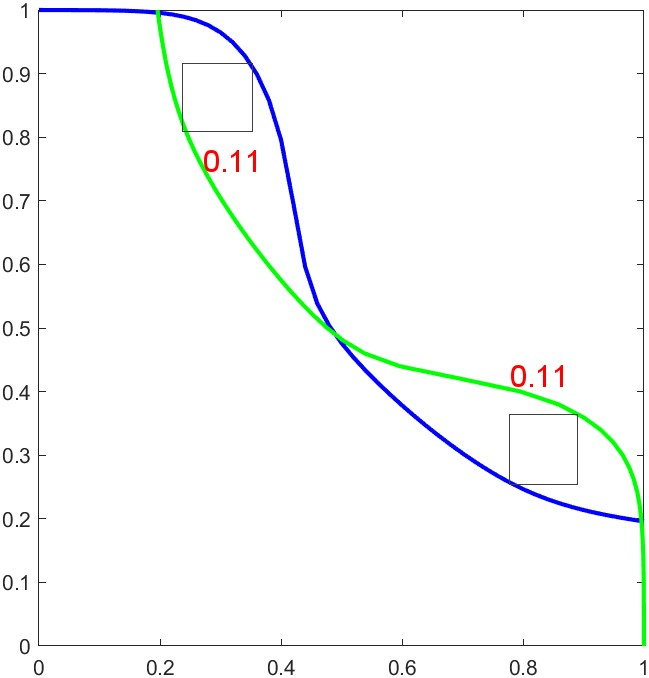
\includegraphics[width=\textwidth]{./img/2023-11-12-01-09-21.png}
\caption{RSNM $V_{DD} = 1V$}
\label{rsnm1}
\end{minipage}
\qquad
\begin{minipage}[t]{0.28\textwidth}
\centering
    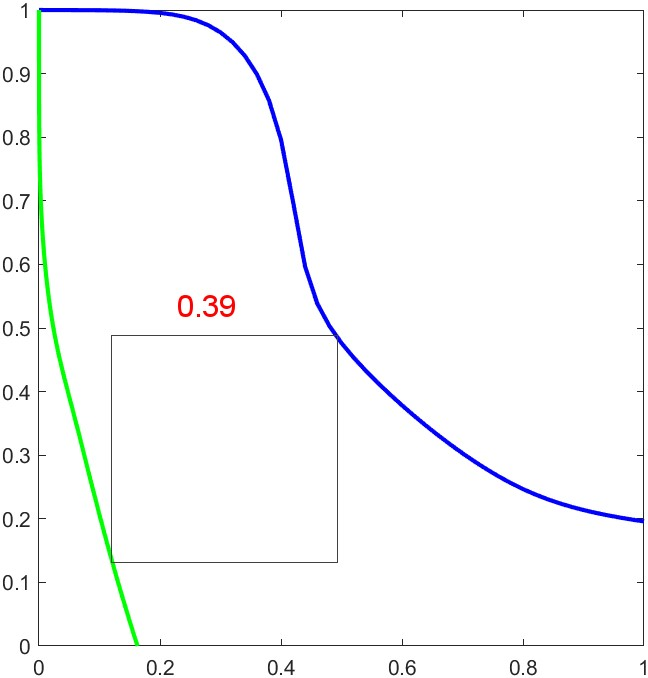
\includegraphics[width=\textwidth]{./img/2023-11-12-01-10-19.png}
\caption{WNM $V_{DD} = 1V$}
\label{wnm1}
\end{minipage}
\end{figure}

\vspace*{-1cm}
對 $V_{DD}$ = 1V, RSNM = 0.156V , WNM = 0.552V

\begin{figure}[H]
\centering
\begin{minipage}[t]{0.28\textwidth}
\centering
    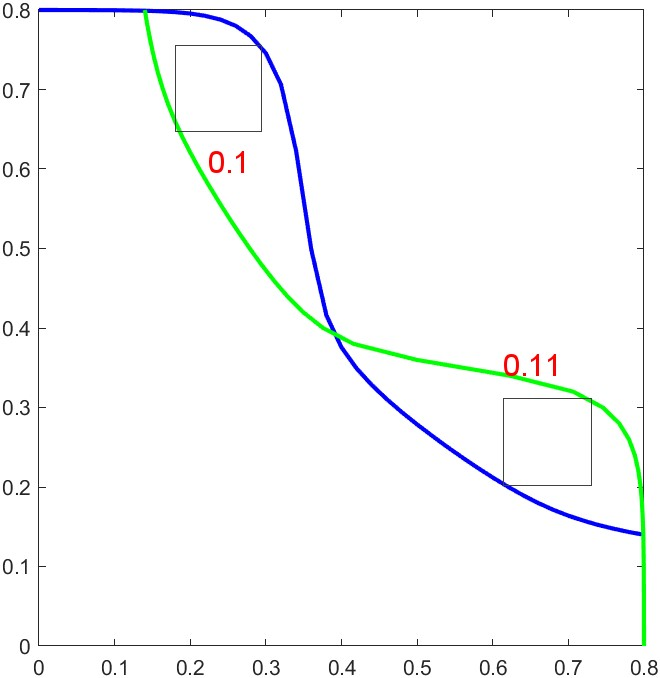
\includegraphics[width=\textwidth]{./img/2023-11-12-01-10-07.png}
\caption{RSNM $V_{DD} = 0.8V$}
\label{rsnm08}
\end{minipage}
\qquad
\begin{minipage}[t]{0.28\textwidth}
\centering
    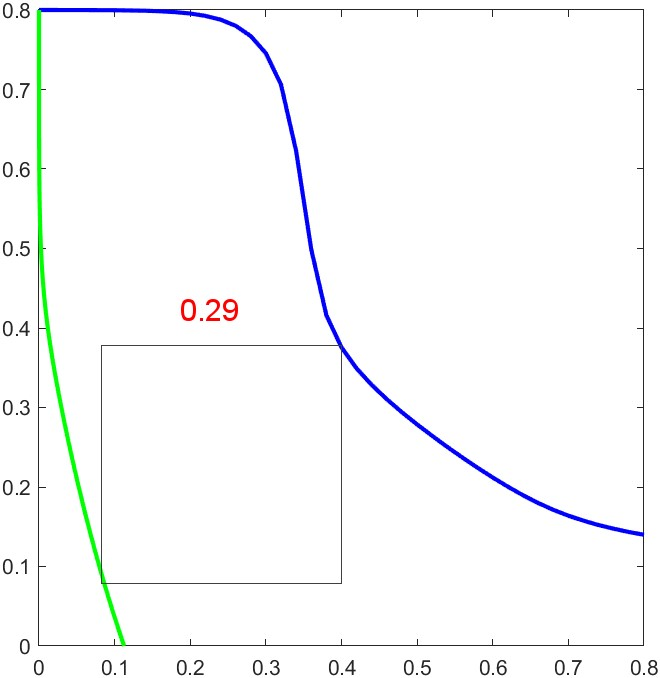
\includegraphics[width=\textwidth]{./img/2023-11-12-01-11-11.png}
\caption{WNM $V_{DD} = 0.8V$}
\label{wnm08}
\end{minipage}
\end{figure}

\vspace*{-1cm}
對 $V_{DD}$ = 0.8V, RSNM = 0.141V , WNM = 0.410V

\begin{figure}[H]
\centering
\begin{minipage}[t]{0.28\textwidth}
\centering
    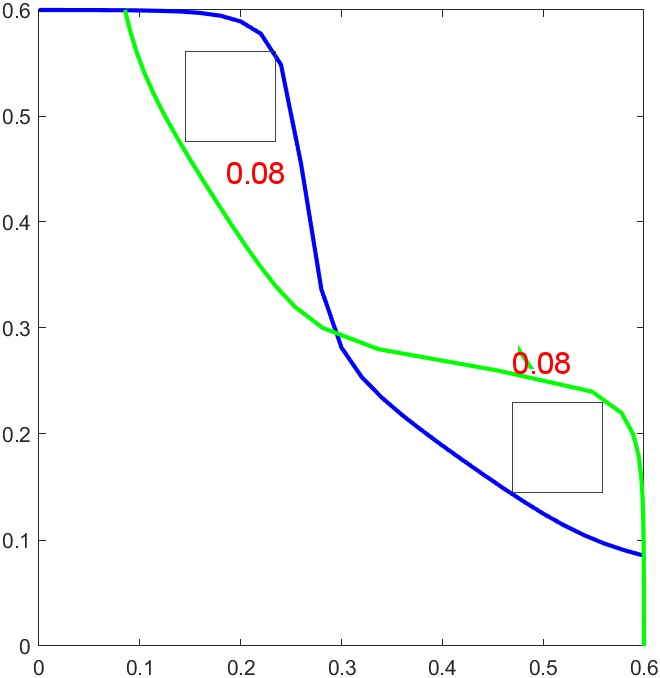
\includegraphics[width=\textwidth]{./img/2023-11-12-01-09-51.png}
\caption{RSNM $V_{DD} = 0.6V$}
\label{rsnm06}
\end{minipage}
\qquad
\begin{minipage}[t]{0.28\textwidth}
\centering
    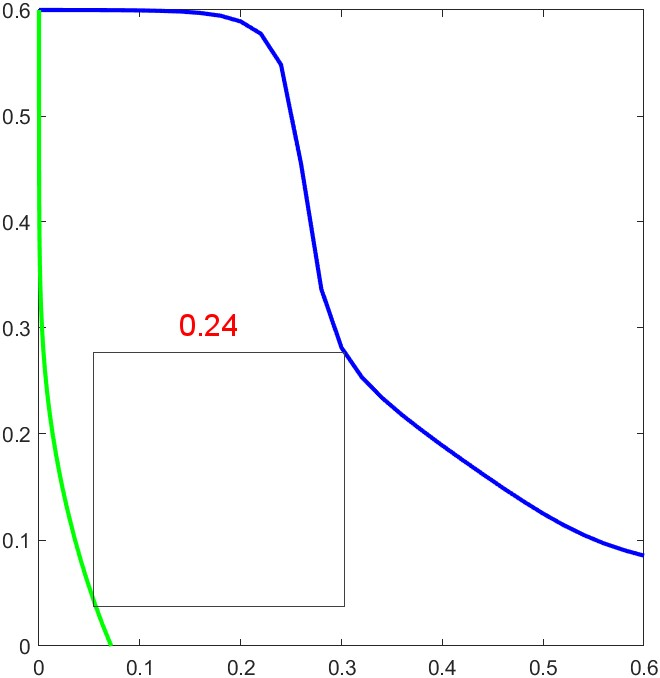
\includegraphics[width=\textwidth]{./img/2023-11-12-01-11-20.png}
\caption{WNM $V_{DD} = 0.6V$}
\label{wnm06}
\end{minipage}
\end{figure}

\vspace*{-1cm}
對 $V_{DD}$ = 0.6V, RSNM = 0.113V , WNM = 0.339V

\begin{figure}[H]
\centering
\begin{minipage}[t]{0.28\textwidth}
\centering
    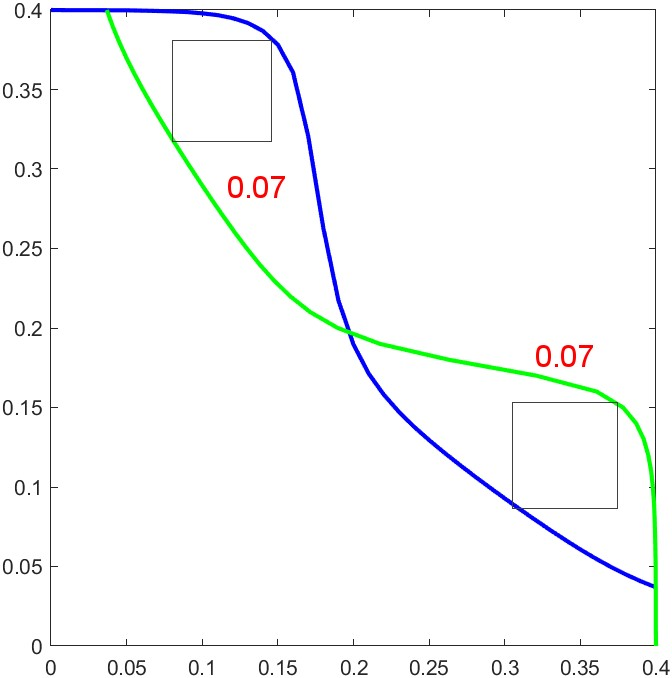
\includegraphics[width=\textwidth]{./img/2023-11-12-01-09-40.png}
\caption{RSNM $V_{DD} = 0.4V$}
\label{rsnm04}
\end{minipage}
\qquad
\begin{minipage}[t]{0.28\textwidth}
\centering
    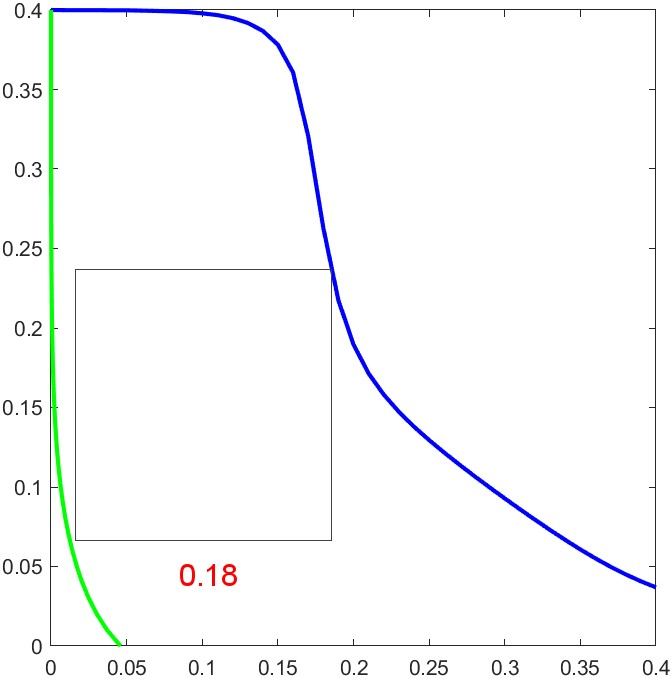
\includegraphics[width=\textwidth]{./img/2023-11-12-01-10-34.png}
\caption{WNM $V_{DD} = 0.4V$}
\label{wnm04}
\end{minipage}
\end{figure}

\vspace*{-1cm}
對 $V_{DD}$ = 0.4V, RSNM = 0.099V , WNM = 0.255V


根據 Fig.\ref{rsnm1}、 Fig.\ref{rsnm08}、 Fig.\ref{rsnm06} 和 Fig.\ref{rsnm04}可以發現RSNM會隨著,VDD變小逐漸變小,與之成正比。而且因為Voltage dividend的關係,在圖形開頭與結尾處會有一個空白區間。根據 Fig.\ref{wnm1}、 Fig.\ref{wnm08}、 Fig.\ref{wnm06} 和 Fig.\ref{wnm04}可以發現WNM也會隨著,VDD變小逐漸變小,與之成正比。通常在同一VDD下, RSNM 都會小於 WNM。


\subsection{8T SRAM}


\begin{figure}[H]
\centering
\begin{minipage}[t]{0.28\textwidth}
\centering
    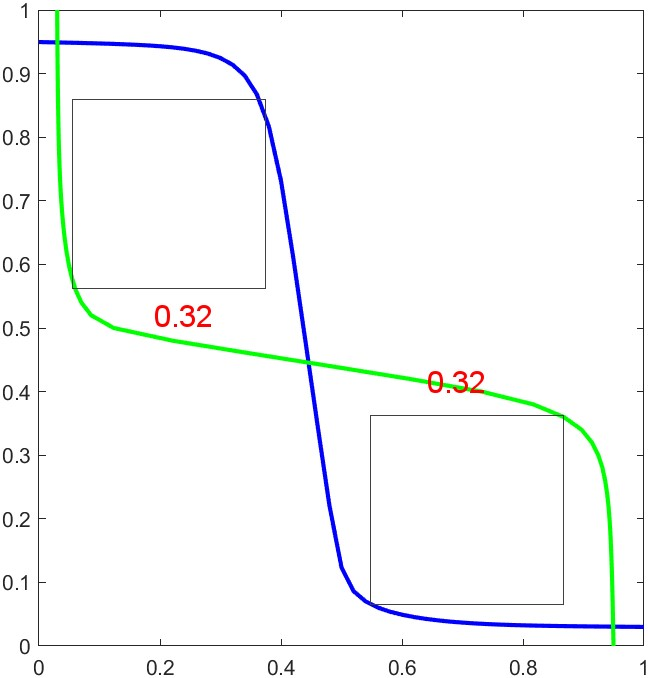
\includegraphics[width=\textwidth]{./img/2023-11-12-04-03-42.png}
\caption{RSNM $V_{DD} = 1V$}
\label{8rsnm1}
\end{minipage}
\qquad
\begin{minipage}[t]{0.28\textwidth}
\centering
    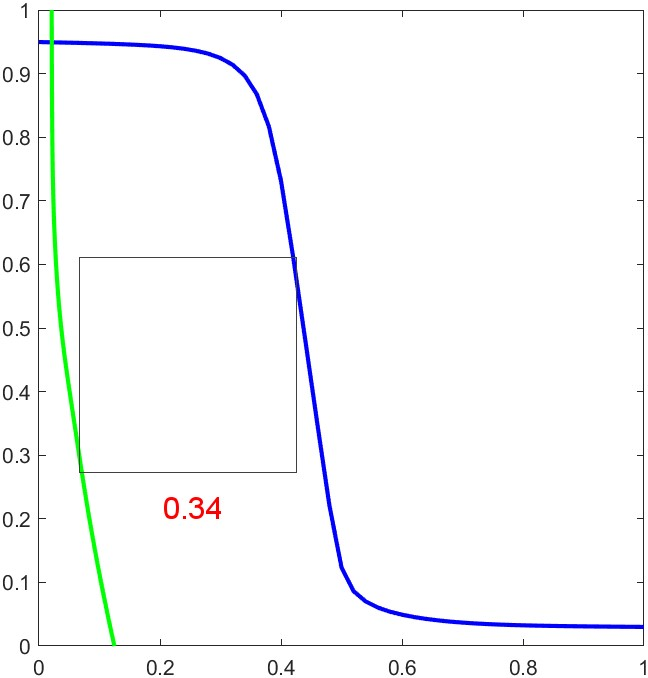
\includegraphics[width=\textwidth]{./img/2023-11-12-04-03-55.png}
\caption{WNM $V_{DD} = 1V$}
\label{8wnm1}
\end{minipage}
\end{figure}

\vspace*{-1cm}
對 $V_{DD}$ = 1V, RSNM = 0.453V , WNM = 0.481V

\begin{figure}[H]
\centering
\begin{minipage}[t]{0.28\textwidth}
\centering
    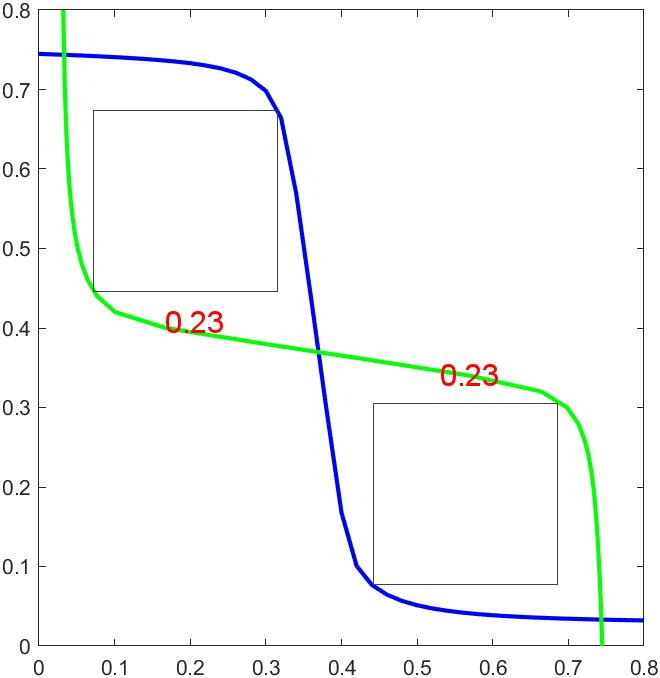
\includegraphics[width=\textwidth]{./img/2023-11-12-04-04-03.png}
\caption{RSNM $V_{DD} = 0.8V$}
\label{8rsnm08}
\end{minipage}
\qquad
\begin{minipage}[t]{0.28\textwidth}
\centering
    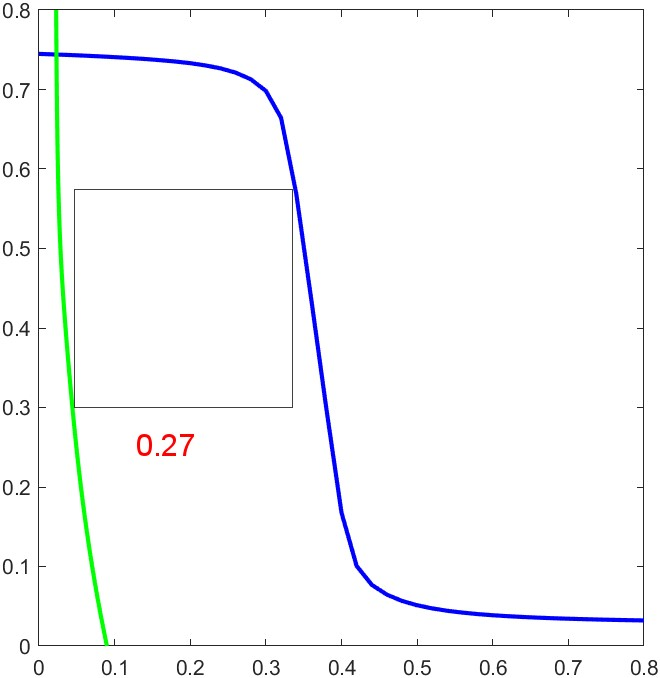
\includegraphics[width=\textwidth]{./img/2023-11-12-04-04-10.png}
\caption{WNM $V_{DD} = 0.8V$}
\label{8wnm08}
\end{minipage}
\end{figure}

\vspace*{-1cm}
對 $V_{DD}$ = 0.8V, RSNM = 0.325V , WNM = 0.382V

\begin{figure}[H]
\centering
\begin{minipage}[t]{0.28\textwidth}
\centering
    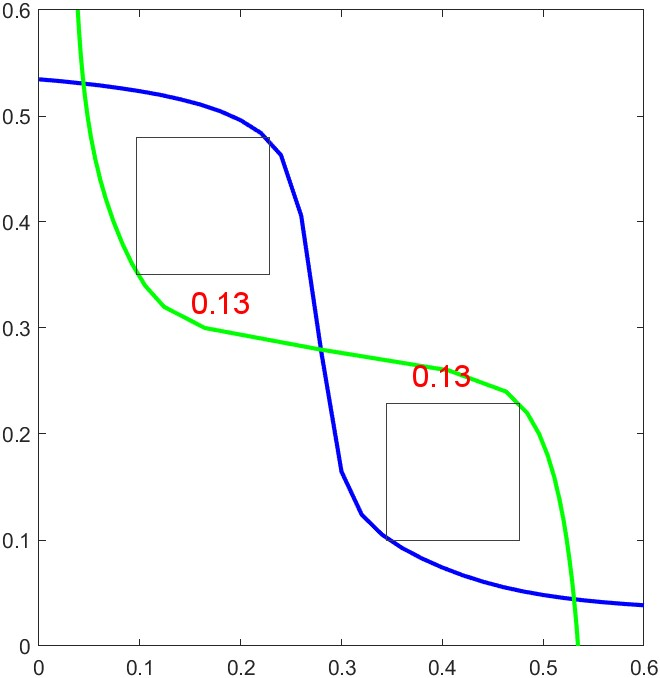
\includegraphics[width=\textwidth]{./img/2023-11-12-04-32-57.png}
\caption{RSNM $V_{DD} = 0.6V$}
\label{8rsnm06}
\end{minipage}
\qquad
\begin{minipage}[t]{0.28\textwidth}
\centering
    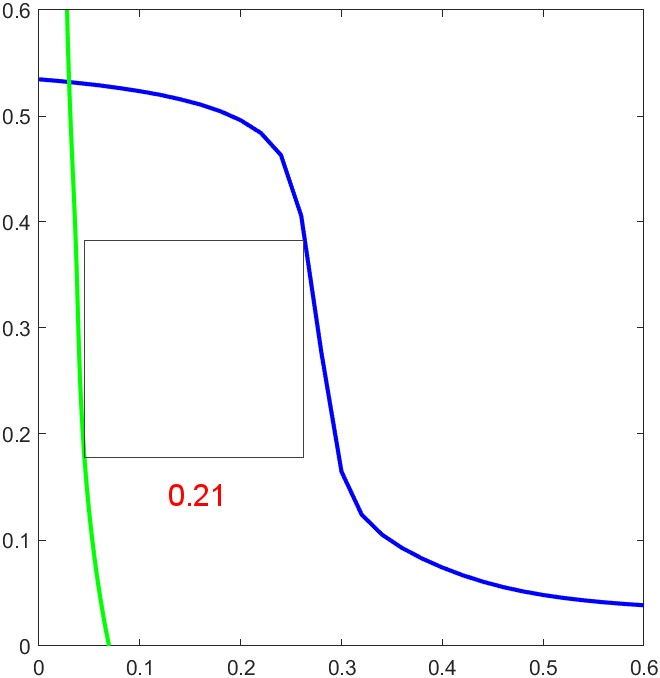
\includegraphics[width=\textwidth]{./img/2023-11-12-04-33-12.png}
\caption{WNM $V_{DD} = 0.6V$}
\label{8wnm06}
\end{minipage}
\end{figure}

\vspace*{-1cm}
對 $V_{DD}$ = 0.6V, RSNM = 0.184V , WNM = 0.297V

\begin{figure}[H]
\centering
\begin{minipage}[t]{0.28\textwidth}
\centering
    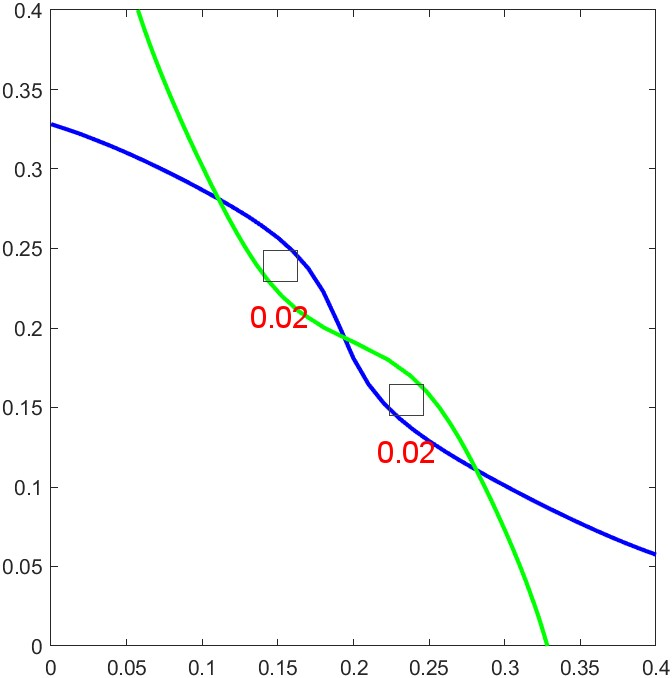
\includegraphics[width=\textwidth]{./img/2023-11-12-04-41-33.png}
\caption{RSNM $V_{DD} = 0.4V$}
\label{8rsnm04}
\end{minipage}
\qquad
\begin{minipage}[t]{0.28\textwidth}
\centering
    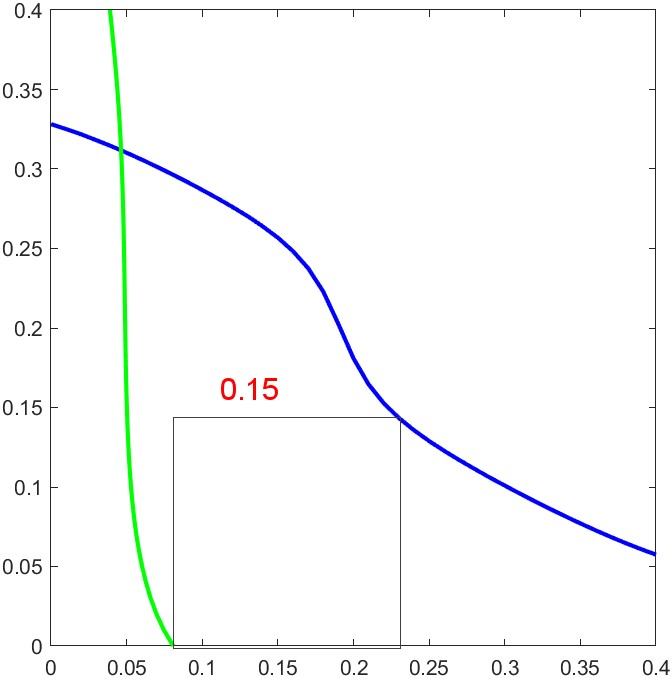
\includegraphics[width=\textwidth]{./img/2023-11-12-04-41-44.png}
\caption{WNM $V_{DD} = 0.4V$}
\label{8wnm04}
\end{minipage}
\end{figure}
    
    \vspace*{-1cm}
    對 $V_{DD}$ = 0.4V, RSNM = 0.028V , WNM = 0.212V
    
    根據 Fig.\ref{8rsnm1}、 Fig.\ref{8rsnm08}、 Fig.\ref{8rsnm06} 和 Fig.\ref{8rsnm04}可以發現RSNM會隨著,VDD變小逐漸變小,與之成正比。而且沒有Voltage dividend的問題,在圖形開頭與結尾無空白區間。根據 Fig.\ref{8wnm1}、 Fig.\ref{8wnm08}、 Fig.\ref{8wnm06} 和 Fig.\ref{8wnm04}可以發現WNM也會隨著,VDD變小逐漸變小,與之成正比。通常在同一VDD下, RSNM 都會小於 WNM。



\section{AC Analysis: Please show the BL (BLB) voltage transient curves of 6T, 8T SRAM during READ and WRITE. You may need toapply appropriate pulses on the WL or BL to READ or to WRITE the cells with VDD=0.8V and the pulse width equivalent to 2ns.}

\subsection{6T SRAM}



\begin{figure}[H]
    \centering
    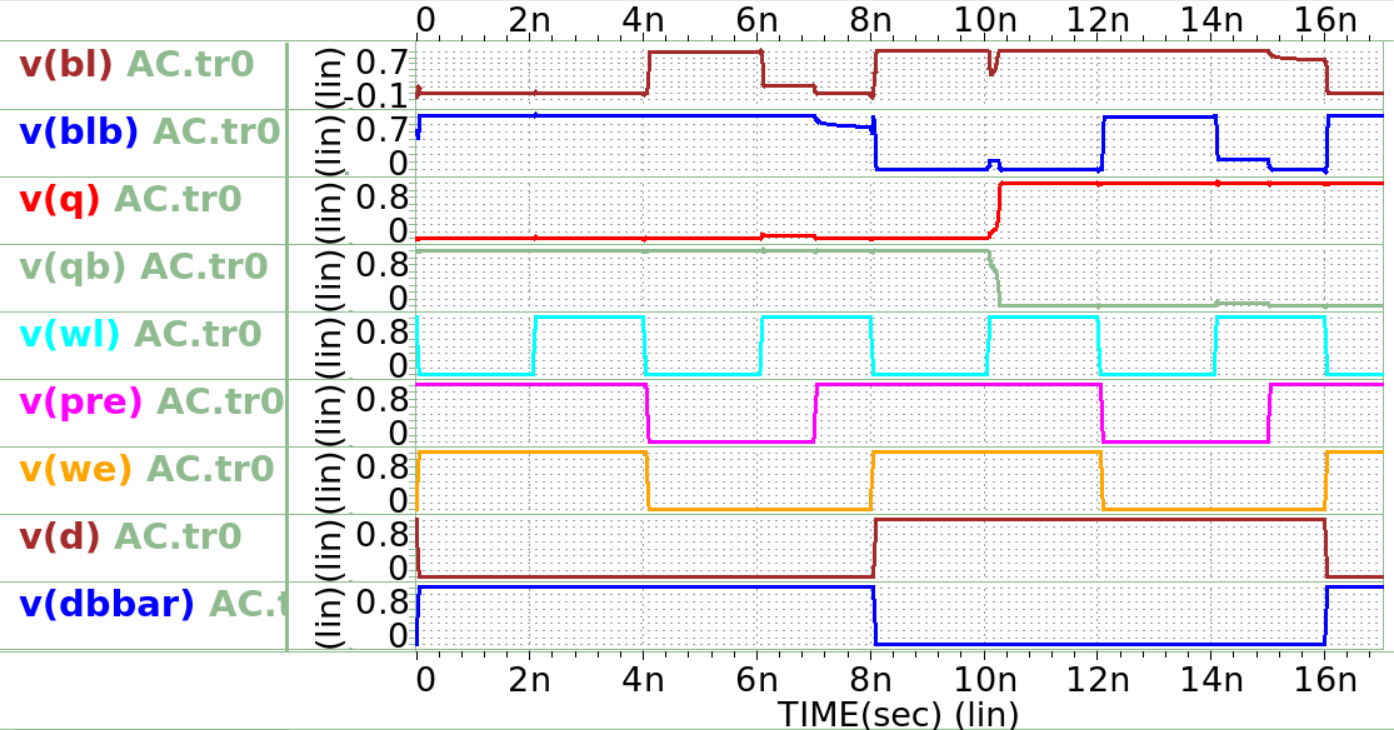
\includegraphics[width=0.9\linewidth]{./img/2023-11-16-09-58-07.png}
    \caption{Transient curves of 6T SRAM}
    \label{tran6T}
    \end{figure}

Fig.\ref{tran6T},操作依序為 WRITE-0、READ-0、WRITE-1、READ-1。\\
v(d) 和 v(dbbar) 分別決定寫入 v(BL) 和 v(BLB) 的值。v(we),是決定寫入d 和 dbar 資訊到 BL 和 BLB。v(pre) 是 Read 之前要先預充電。以下Fig.\ref{6T1} - Fig.\ref{6T4}為分段解釋。

\begin{figure}[H]
    \centering
    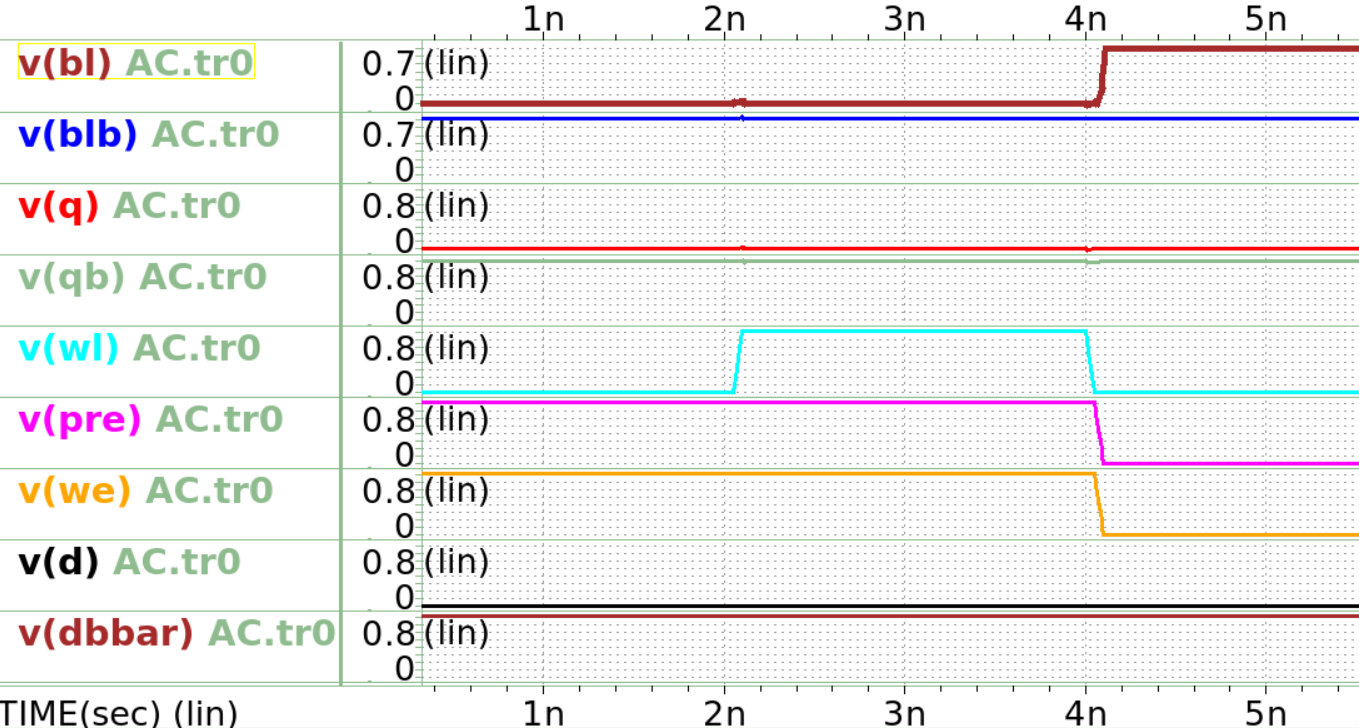
\includegraphics[width=0.7\linewidth]{./img/2023-11-16-12-53-45.png}
\caption{6T SRAM Write-0}
\label{6T1}
\end{figure}

Fig.\ref{6T1},在寫入值時,不需要 precharge 所以 v(pre) 為 VDD (pmos off)。\\v(d) = 0、v(dbbar) = VDD 才能寫0進去。


\begin{figure}[H]
\centering
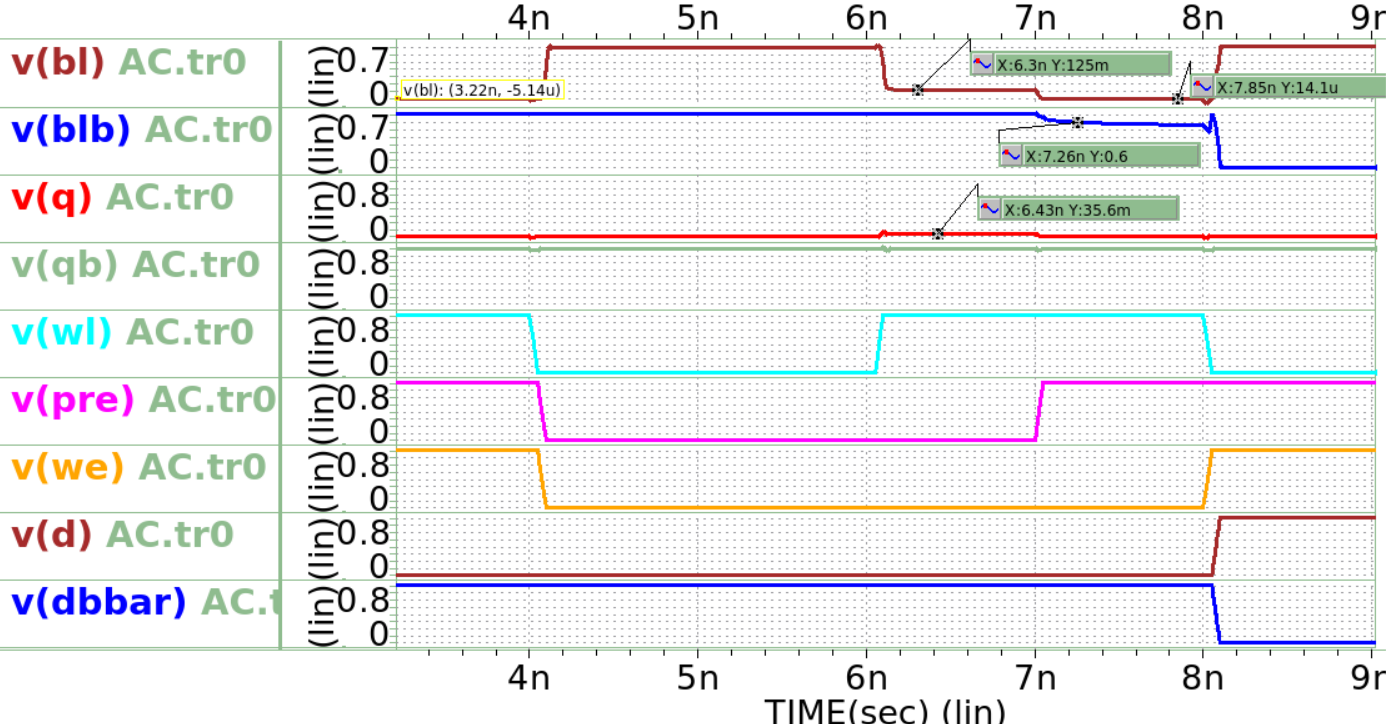
\includegraphics[width=0.7\linewidth]{./img/2023-11-16-10-05-30.png}
\caption{6T SRAM Read-0}
\label{6T2}
\end{figure}

Fig.\ref{6T2},在讀取值時,需要 precharge 所以 v(pre) 為 0 (pmos on)。v(d)。 v(pre) 在 6T SRAM 為寫入狀態持續打開的話,會影響到電壓 v(BL) 會變得大一點,但不影響讀取。

\begin{figure}[H]
\centering
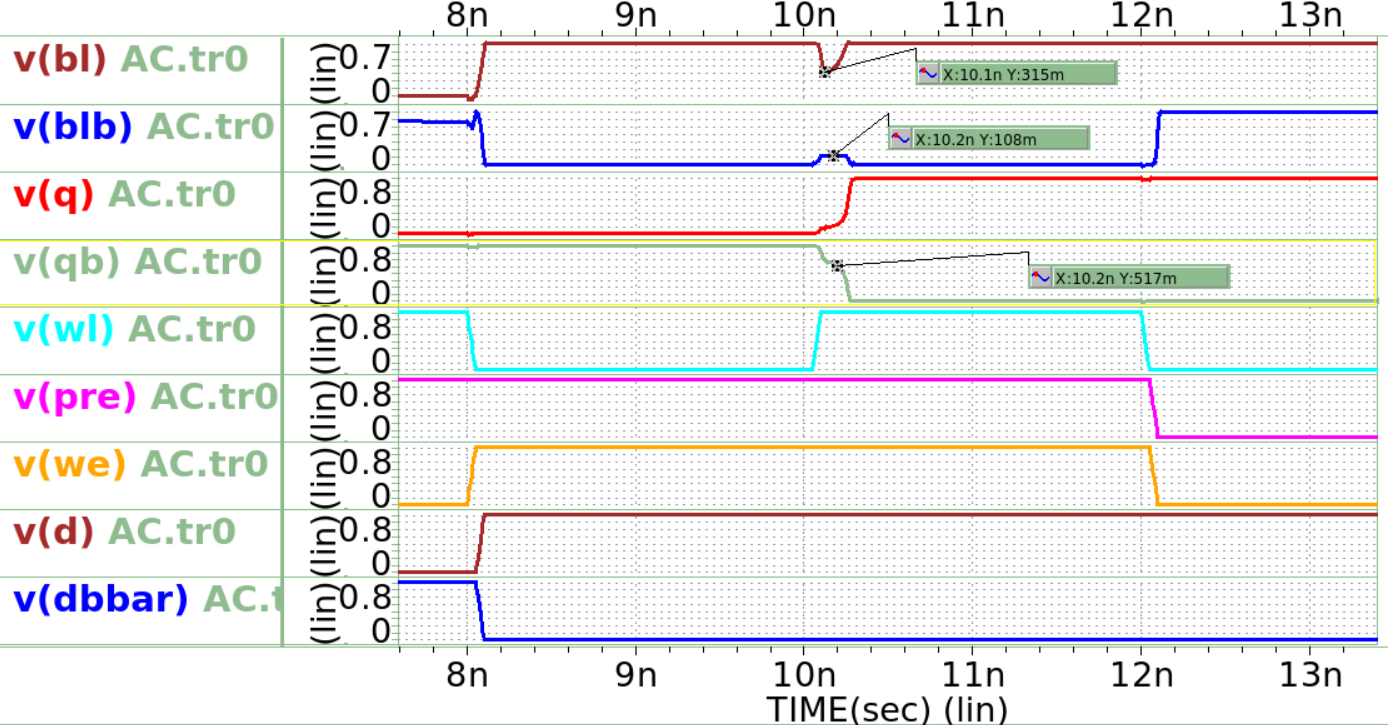
\includegraphics[width=0.7\linewidth]{./img/2023-11-16-10-06-40.png}
\caption{6T SRAM Write-1}
\label{6T3}
\end{figure}

Fig.\ref{6T3},在寫入值時,不需要 precharge 所以 v(pre) 為 VDD (pmos off)。\\v(d) = VDD、v(dbbar) = 0 才能寫 1 進去。

\begin{figure}[H]
\centering
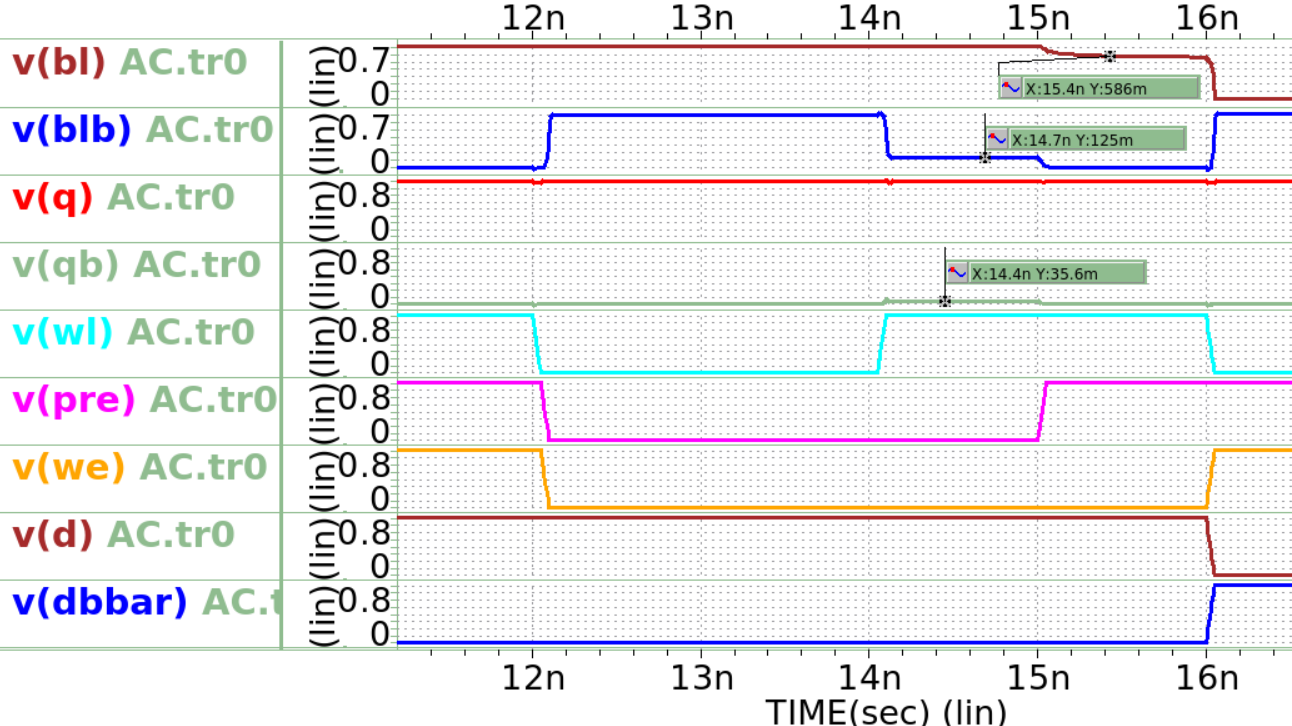
\includegraphics[width=0.7\linewidth]{./img/2023-11-16-10-08-04.png}
\caption{6T SRAM Read-1}
\label{6T4}
\end{figure}

Fig.\ref{6T4},在讀取值時,需要 precharge 所以 v(pre) 為 0 (pmos on)。v(d)。 v(pre) 在 6T SRAM 為寫入狀態持續打開的話,會影響到電壓 v(BLB) 會變得大一點,但不影響讀取。




\subsection{8T SRAM}

\begin{figure}[H]
\centering
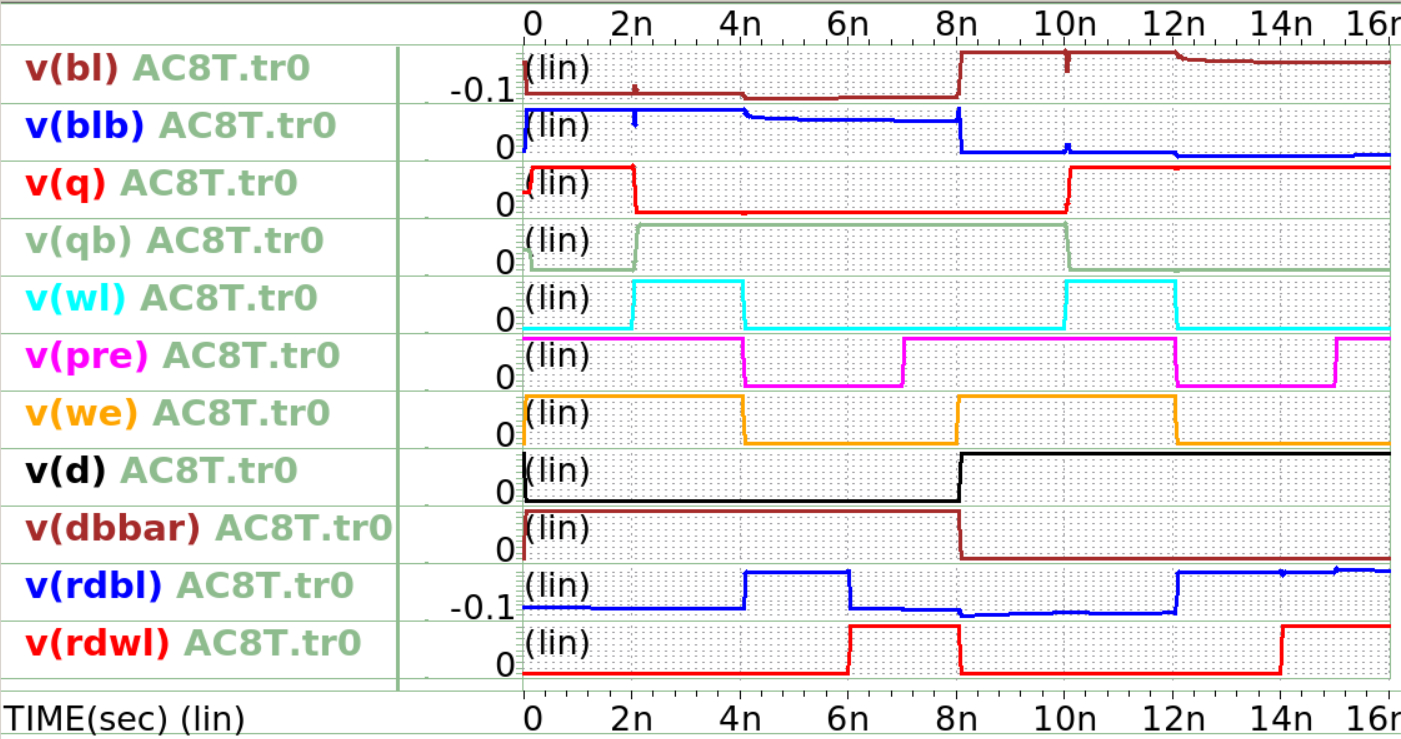
\includegraphics[width=\linewidth]{./img/2023-11-16-13-30-04.png}
\caption{Transient curves of 8T SRAM}
\label{tran8T}
\end{figure}

Fig.\ref{tran8T},操作依序為 WRITE-0、READ-0、WRITE-1、READ-1。\\
v(d) 和 v(dbbar) 分別決定寫入 v(BL) 和 v(BLB) 的值。v(we),是決定寫入d 和 dbar 資訊到 BL 和 BLB。v(pre) 是 Read 之前要先預充電。r(rdwl) 決定是否要讀取,r(rdbl)為讀取出來的電壓值。

\begin{figure}[H]
\centering
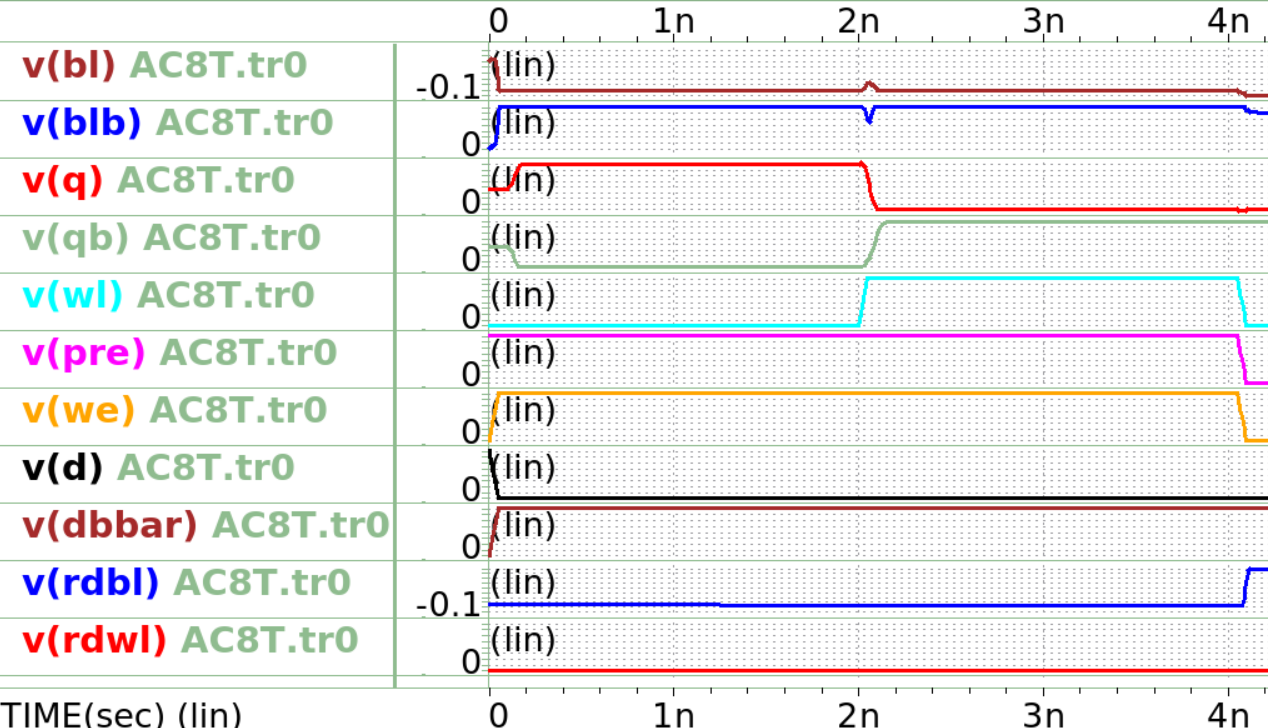
\includegraphics[width=0.7\linewidth]{./img/2023-11-16-13-35-03.png}
\caption{8T SRAM Write-0}
\label{8T1}
\end{figure}

\vspace*{-1em}

Fig.\ref{8T1},在寫入值時,不需要 precharge 所以 v(pre) 為 VDD (pmos off)。\\v(d) = 0、v(dbbar) = VDD 才能寫0進去。

\begin{figure}[H]
\centering
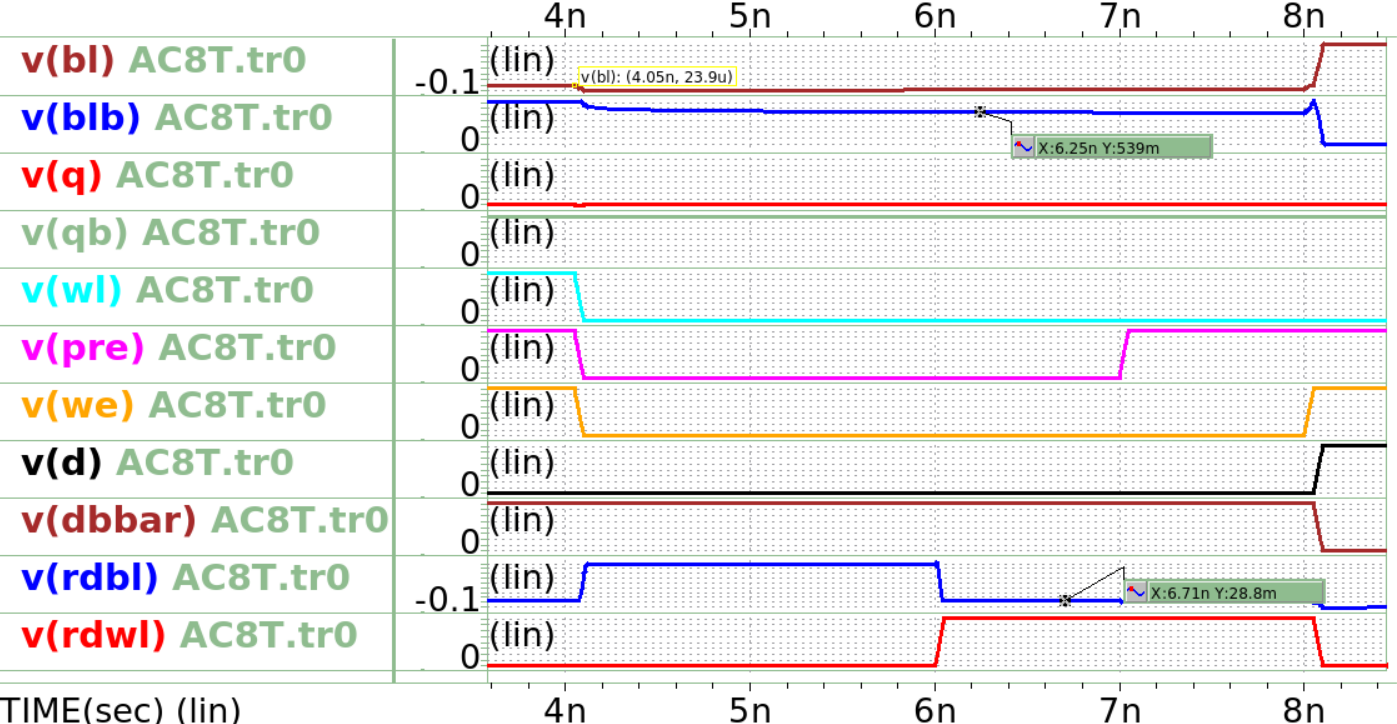
\includegraphics[width=0.7\linewidth]{./img/2023-11-16-13-34-20.png}
\caption{8T SRAM Read-0}
\label{8T2}
\end{figure}

Fig.\ref{8T2},在讀取值時,需要 precharge 所以 v(pre) 為 0 (pmos on)。v(we) 關閉,會影響到電壓 v(BLB) 會掉一點,但不影響讀取。

\begin{figure}[H]
\centering
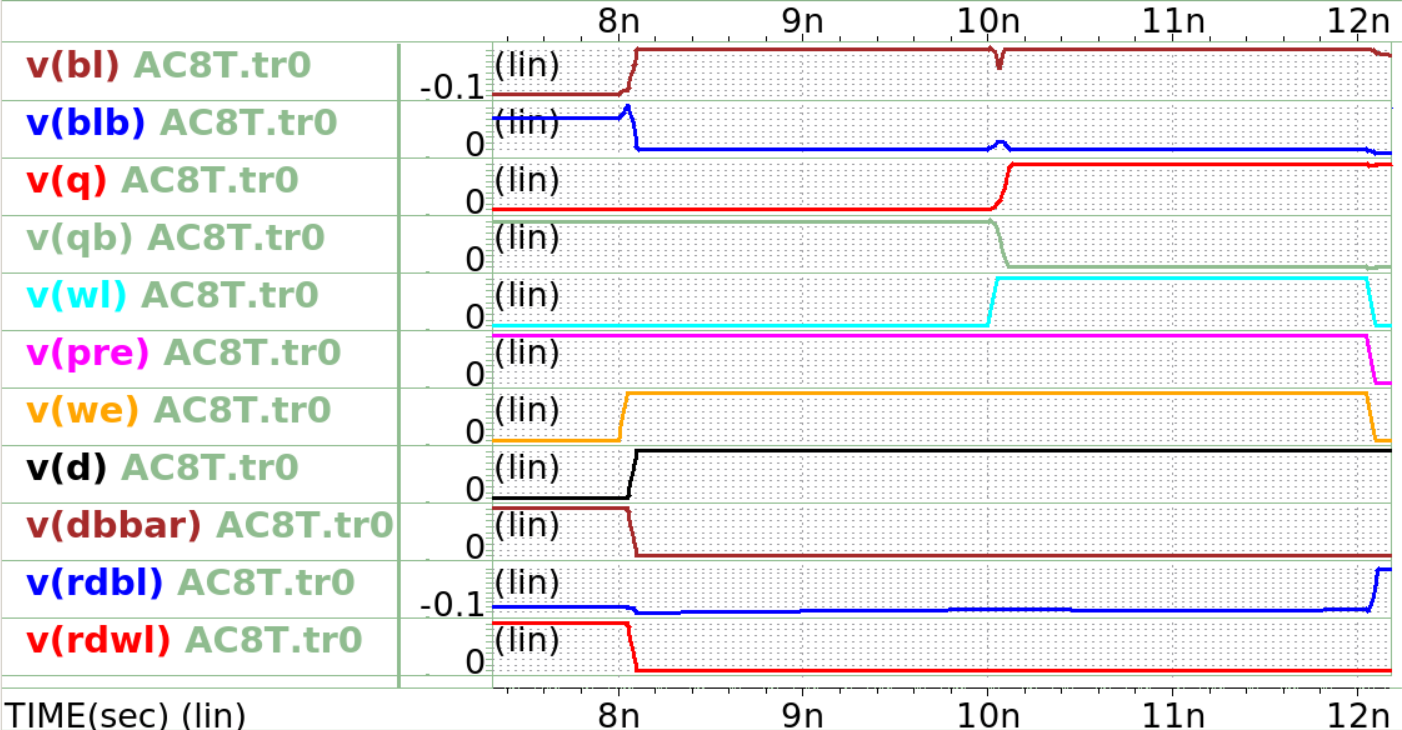
\includegraphics[width=0.7\linewidth]{./img/2023-11-16-13-36-04.png}
\caption{8T SRAM Write-1}
\label{8T3}
\end{figure}

Fig.\ref{8T3},在寫入值時,不需要 precharge 所以 v(pre) 為 VDD (pmos off)。\\v(d) = VDD、v(dbbar) = 0 才能寫1進去。

\begin{figure}[H]
\centering
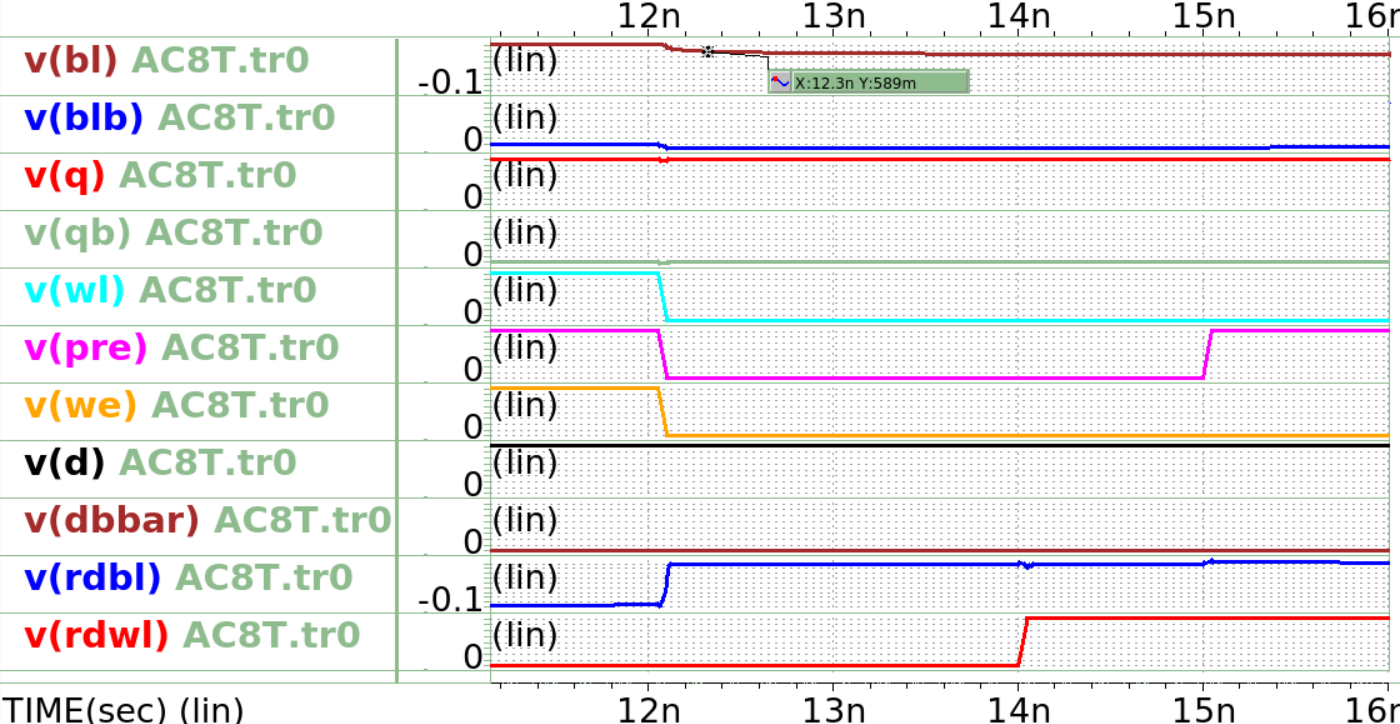
\includegraphics[width=0.7\linewidth]{./img/2023-11-16-13-37-07.png}
\caption{8T SRAM Read-1}
\label{8T4}
\end{figure}

Fig.\ref{8T4},在讀取值時,需要 precharge 所以 v(pre) 為 0 (pmos on)。v(we) 關閉,會影響到電壓 v(BL) 會掉一點,但不影響讀取。

\section{Power Analysis: Please show the BL (BLB) power transient curves of 6T, 8T SRAM during READ and WRITE. The powertransient curves can be calculated by multiplication of voltage and current transient curves. (P=IxV) You may need to applyappropriate pulses on the WL or BL to READ or to WRITE the cells with VDD=0.8V and the pulse width equivalent to 2ns.}

\begin{figure}[H]
\centering
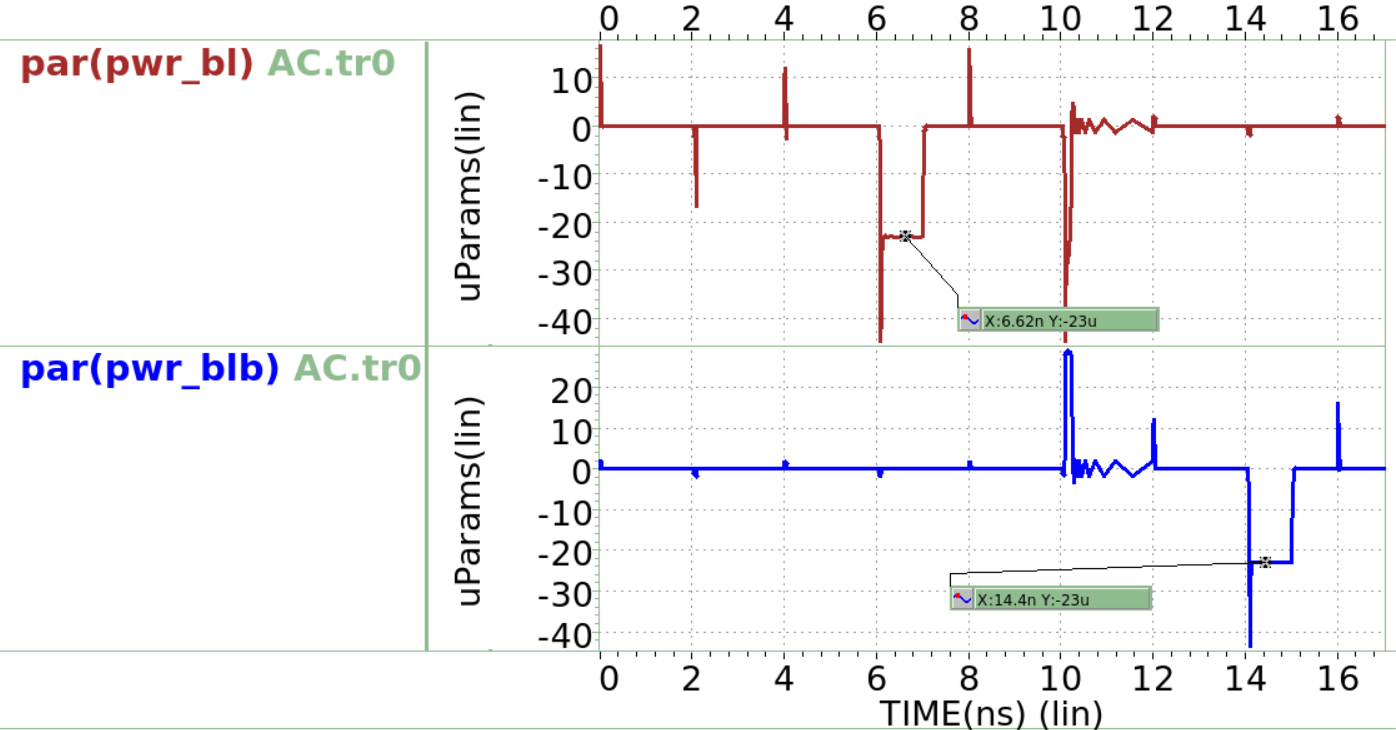
\includegraphics[width=\linewidth]{./img/2023-11-16-09-11-23.png}
\caption{6T SRAM}
\label{p6T}
\end{figure}

根據 Fig.\ref{p6T},當 v(WL)、v(BL)和v(BLB),有變動,會影響到 Power,可見讀寫線合一。圖上 Label 的小電流是 precharge 充電,同時讀取帶來的小電流所以有 Power。
   

\begin{figure}[H]
    \centering
    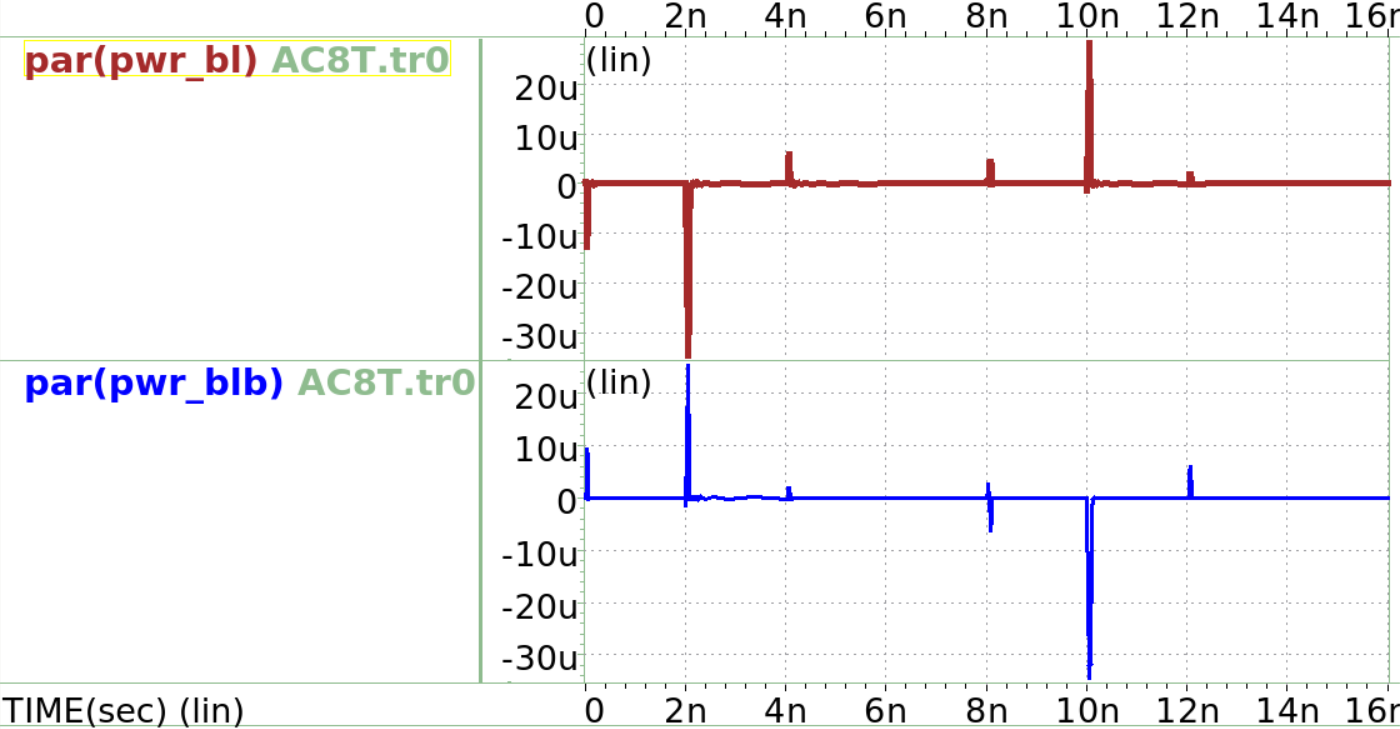
\includegraphics[width=\linewidth]{./img/2023-11-16-13-29-31.png}
    \caption{8T SRAM}
\label{p8T}
    \end{figure}
    
根據 Fig.\ref{p8T},只有當 v(WL)、v(BL)和v(BLB),有變動,才會影響到 Power。v(rdbl) 和 v(rdwl) 變動不會影響其 Power,可見讀寫線分離。
   

\section{參考資料}

\begin{enumerate}

\item\href{https://citeseerx.ist.psu.edu/viewdoc/download;jsessionid=151FCDB529E9C1DDACEFF440EBB2194A?doi=10.1.1.679.5935&rep=rep1&type=pdf}{SNM Analysis of Sram Cells at 45nm, 32nm and 22nm Technology}

\item\href{http://163.17.20.49/AIT2011/2011AIT%E8%AB%96%E6%96%87%E5%85%A8%E6%96%87/ft_145.pdf}{A Low Power and High Read Stability SRAM
Cell Using Single-ended Bit-line }

\item\href{https://github.com/Hassan313/Near-Threshold-SRAM/blob/master/SRAM%20Cells%20Netlist/8T_SRAM_Cell.sp}{Near-Threshold-SRAM}

\item\href{https://www.researchgate.net/publication/303563712_An_efficient_timing_analysis_model_for_6T_FinFET_SRAM_using_current-based_method}{An efficient timing analysis model for 6T FinFET SRAM using current-based method}

\item\href{https://zheliu0.com/post/sram/}{1-Bit SRAM Cell in 45-nm CMOS Technology with Integrated Dynamic Power Supply}
 
\end{enumerate}

\end{document}